\documentclass[xcolor=dvipsnames,10pt]{beamer}

\mode<presentation> {\usetheme{Singapore}}
\usepackage{pgfpages}

%\setbeamercovered{transparent} 
\usepackage[english]{babel}
\usepackage[latin1]{inputenc}
\usepackage{times,amsfonts}
\usepackage[T1]{fontenc}
\setlength{\parskip}{\baselineskip}
% Or whatever. Note that the encoding and the font should match. If T1
% does not look nice, try deleting the line with the fontenc.

%\usecolortheme{sidebartab}
\setbeamertemplate{itemize item}[triangle]



\usepackage{calc}
\usepackage{environ}
\newcommand{\halfmargin}{0.0001\paperwidth}


\RequirePackage{booktabs,colortbl,ulem}

\usepackage{animate}
\RequirePackage{booktabs,colortbl,gensymb}
\setlength{\parskip}{\baselineskip}

\usepackage{calc}
\usepackage{environ}

% \newcommand{\halfmargin}{0.0001\paperwidth}


\NewEnviron{wideframe}[1][]{%
\begin{frame}{#1}
\makebox[\textwidth][c]{
\begin{minipage}{\dimexpr\paperwidth-\halfmargin-\halfmargin\relax}
\BODY
\end{minipage}}
\end{frame}
}


\DeclareMathOperator{\stdev}{stdev}
\DeclareMathOperator{\var}{var}
\DeclareMathOperator{\cov}{cov}
\DeclareMathOperator{\corr}{corr}
\DeclareMathOperator{\prob}{prob}
\DeclareMathOperator{\n}{n}
\DeclareMathOperator{\N}{N}
\DeclareMathOperator{\Cov}{Cov}

\newcommand{\hlf}{\frac{1}{2}}
\newcommand{\bi}{\begin{itemize}}
\newcommand{\ei}{\end{itemize}}
\newcommand{\im}{\item}
\newcommand{\D}{\mathrm{d}}
\newcommand{\E}{\mathrm{e}}
\newcommand{\mye}{\ensuremath{\mathsf{E}}}
\newcommand{\myreal}{\ensuremath{\mathbb{R}}}
\newcommand{\bq}{\begin{equation}}
\newcommand{\eq}{\end{equation}}
\newcommand{\eqdef}{\;\buildrel \text{d{}ef}\over = \;}
\newcommand{\xstar}{\buildrel *\over X}
\newcommand{\pmax}{p^{\text{max}}}
\newcommand{\qmax}{q^{\text{max}}}
\newcommand{\bfr}{\begin{frame}}
\newcommand{\bfrp}{\begin{frame}[plain]}
\newcommand{\efr}{\end{frame}}
\newcommand{\F}{\mathcal{F}}
\newcommand{\FF}{\mathbb{F}}
\newcommand{\ve}{\varepsilon}
\newcommand{\lh}{\hat{\lambda}}
\definecolor{mycolor}{gray}{0.8}
\definecolor{mymaincolor}{rgb}{0.6862745098039216,0.9333333333333333,0.9333333333333333}
\newcommand{\alr}[1]{\textcolor{blue}{#1}}
\definecolor{LightCyan}{rgb}{0.88,1,1}
\newcommand{\yel}{\cellcolor{yellow}}
\newcommand{\blue}{\cellcolor{SkyBlue}}
\newcommand{\gr}{\cellcolor{SpringGreen}}
\newcommand{\pink}{\cellcolor{pink}}
\newcommand{\apr}{\cellcolor{Apricot}}
\newcommand{\tve}{\tilde{\varepsilon}}
\newcommand{\tw}{\tilde{w}}
\newcommand{\ttth}{\tilde{\theta}}
\newcommand{\te}{\tilde{e}}
\newcommand{\ts}{\tilde{s}}
\newcommand{\tx}{\tilde{x}}
\newcommand{\ty}{\tilde{y}}
\newcommand{\tv}{\tilde{v}}
\newcommand{\tp}{\tilde{p}}
\newcommand{\tF}{\tilde{F}}
\newcommand{\tf}{\tilde{f}}
\newcommand{\tZ}{\tilde{Z}}
\newcommand{\ow}{\overline{w}}
\newcommand{\lb}{\left[}
\newcommand{\rb}{\right]}
\newcommand{\lp}{\left(}
\newcommand{\rp}{\right)}
\newcommand{\tm}{\tilde{m}}
\newcommand{\tc}{\tilde{c}}
\newcommand{\tz}{\tilde{z}}
\newcommand{\str}[1]{\textcolor{blue}{\sout{#1}}}
\newcommand{\tr}{\widetilde{R}}
\newcommand{\tR}{\widetilde{\mathbf{R}}}
\newcommand{\bms}{\begin{multline*}}
\newcommand{\ems}{\end{multline*}}
\newcommand{\bas}{\begin{align*}}
\newcommand{\eas}{\end{align*}}
\newcommand{\qr}{\mathbb{Q}}
\newcommand{\IMAGES}{/home/kerry/Dropbox/Images}
\newcommand{\tX}{\tilde{X}}
\newcommand{\tY}{\tilde{Y}}

\author{\vskip 0.5in \small Kerry Back \\BUSI 521--ECON 505\\ Rice University \\Spring 2022}
%\institute{Rice University\\ Spring 2019}
\date[]





\newcommand{\tu}{\tilde{u}}
\begin{document}
\title{\vskip 0.5in Day 15}
\subtitle{Market Microstructure}

\begin{frame}
  \titlepage
\end{frame}

\section{Order-Driven Market}\subsection{}

\bfr\frametitle{Kyle Model}

Similar structure to Grossman-Stiglitz model: one risky asset, risk-free asset, informed and uninformed investors.

But only one informed investor.

And, everyone is risk neutral.

Informed investor submits an order $\tu$.  Simultaneously, noise (liquidity) traders submit an order $\tz$.  Assume

Rest of market (market makers) see $\ty := \tu+\tz$.  Update beliefs.  Equilibrium price is expected asset value conditional on $\ty$ discounted at the risk-free rate.
\end{frame}

\begin{frame}{Equilibrium}
    Assume the asset value $\tx$ and signal signal $\ts$ are as in Grossman-Stiglitz model.  Posterior mean for informed is $(1-\beta)\mu + \beta \ts$.
        Set 
    $$\tv = \frac{(1-\beta)\mu + \beta\ts}{R_f}$$
        Equilibrium means
    \vspace*{-\baselineskip}
    \begin{itemize}
    \item  $p=\mye[\tv \mid \ty]$ given the informed strategy (which determines the information in $\ty$) and 
    \item the informed strategy is optimal given the market makers' pricing rule (which determines how $p$ depends on $\ty$)
    \end{itemize}
    
    There is an equilibrium with \vspace*{-\baselineskip}
    \begin{itemize}
        \item $p = \mu/R_f + \lambda \ty$ for a constant $\lambda$ (called Kyle's lambda)
        \item $\tu = \delta(\ts - \mu)$ for a constant $\delta$
    \end{itemize}
    

\end{frame}




\bfr\frametitle{Proof}
Given $\ty = \delta(\ts-\mu)+\tz$, compute $p=\mye[\tv\mid \ty]$ by projection of $\tv$ on $\ty$.  Get a linear relation depending on $\delta$.

The informed trader chooses $u$, given $v$, to maximize
$$\mye[(v-p)u] = \my\big[\big(v-\mu/R_f-\lambda(u+\tz)\big)u\big] = \big(v-\mu/R_f-\lambda u\big)u$$
Get a linear relation between $u$ and $v$ depending on $\lambda$.

Combining these, we get $\delta \mapsto \lambda \mapsto \delta$ with everything linear and a unique fixed point (just solve a linear equation).
\end{frame}

\begin{frame}{Properties}
Denote the prior variance of $\tv$ by $\sigma_v^2$.  The posterior variance given the information in $\tu$, equivalently the information in $p$, is $\sigma_v^2/2$.  Half of the uncertainty is resolved.

Kyle's lambda is $\sigma_v/(2\sigma_z)$. Kyle calls $1/\lambda$ the depth of the market.  It is the number of shares you can trade with a \$1 effect on the price.

The market is deeper 
\vspace*{-0.5\baselineskip}
\begin{itemize} 
\item when there is more noise trading ($\sigma_z$ is larger),
\item when there is less asymmetric information ($\sigma_v$ is smaller).
\end{itemize}
    The informed trader's expected profit is $\sigma_v\sigma_z$.  This is also the expected loss of noise traders.  Market makers break even on average.
\end{frame}


\section{Quote-Driven Markets}\subsection{}

\begin{frame}{Glosten-Milgrom Model}
    Glosten and Milgrom assume risk-neutral market makers set bid and ask prices $b<a$ first.
    
    Then a trader arrives (either informed or uninformed) and trades 1 share, either buying or selling.
    
    Example: asset value $\tv$ is either 0 or 1.  Uninformed traders are equally likely to buy or to sell, regardless of the bid and ask prices.
    
    Informed trader will buy and earn $1-a$ if the value is 1 and sell and earn $b$ if the value is 0.
    
    Suppose probability of an informed trader is $\pi$ independent of the bid and ask, and denote probability $\tv=1$ by $\delta$. 
\end{frame}

\begin{frame}{Equilibrium}
Probability of informed buy conditional on buy is 
$$p(\text{informed buy}\mid \text{buy} = )\frac{p(\text{informed buy})}{p(\text{buy})} = \frac{\pi \delta}{(1-\pi)/2 + \pi\delta} $$
Ask price is
\begin{align*}
\mye[\tv \mid \text{buy}] &= \mye[\tv \mid \text{informed buy}]p(\text{informed buy}\mid \text{buy}) \\ 
    &\qquad + \mye[\tv \mid \text{uninformed buy}]p(\text{uninformed buy}\mid \text{buy}) \\ 
    & = 1 \times \frac{\pi \delta}{(1-\pi)/2 + \pi\delta} + \frac{1}{2} \times \frac{(1-\pi)/2}{(1-\pi)/2 + \pi\delta}
\end{align*}
Symmetrically, bid price is
\begin{align*}
    \mye[\tv \mid \text{sell}] &= \mye[\tv \mid \text{informed sell}]p(\text{informed sell}\mid \text{sell}) \\
    & \qquad + \mye[\tv \mid \text{uninformed sell}]p(\text{uninformed sell}\mid \text{sell}) 
    \\ &= 0 \times \frac{\pi (1-\delta)}{(1-\pi)/2 + \pi(1-\delta)} + \frac{1}{2} \times \frac{(1-\pi)/2}{(1-\pi)/2 + \pi(1-\delta)}
\end{align*}
    \end{frame}
\begin{frame}{Properties}
    Suppose this process is repeated for $T$ periods with $\delta$ (prob $\tv=1$) adjusting as orders arrive.
    
    The sequence of transaction prices is a martingale.  Transaction prices are conditional expectations of $\tv$, conditioning on more information over time.
    
    So, price changes have zero correlation.
    
    Also, the price at $T$ will be close to $\tv$ if $T$ is large.
\end{frame}

\section{Limit-Order Markets}\subsection{}

\begin{frame}{Auctions versus Limit-Order Markets}
The title of Kyle's paper is `Continuous Auctions and Insider Trading.'

In an auction, something is offered for sale and people bid for it, either simultaneously (sealed bid) or with an ascending or descending price (open outcry).

In the Kyle model, the net excess demand $\ty$ is offered to the market makers and they bid to supply it (if $\ty>0$) or buy it (if $\ty<0$), so it is an auction. 

In auction theory, the bidders are assumed to have diverse information.  That's what makes it interesting.  In Kyle's model, the bidders are uninformed, so it is a Bertrand game.

Modern markets are mostly organized as open limit-order books.  Limit-order markets are not auctions.

\end{frame}

\bfr{Snapshot of a Limit Order Book}
 \vspace*{-0.1in}
 \begin{center}
 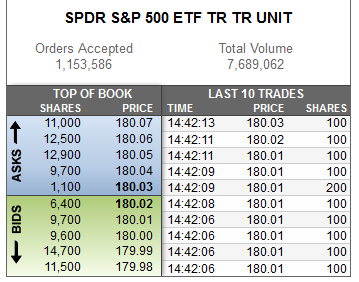
\includegraphics[scale=0.4]{Images/LOB.png}
 \end{center}
 \vspace*{-0.25in}\small

 A newly arriving order will either go into the book or (if ``marketable'') be executed against orders already in the book.  Marketable orders 'walk up' or 'walk down' the book, executing at the limit prices of orders already in the book.  The total cost paid (received) is the area under the supply (demand) curve.
 \end{frame}

\begin{frame}{Equilibrium in a Static Model}
    Assume competitive risk-neutral market makers submit limit orders.
    A market order will arrive from an informed or uninformed trader of variable size.
    
    Equilibrium prices are similar to Glosten-Milgrom: expected values conditional on trade.
    
 Your limit order executes when there is a market order large enough to wipe out the limit orders ahead of you and hit your limit order.
 
 So, equilibrium prices are `tail expectations.'  Bids are $$\mye[\tv | \text{sell} >= \text{number of orders at higher bids}$$
 Asks are
 $$\mye[\tv | \text{buy} >= \text{number of orders at lower asks}$$
 \end{frame}

\bfr\frametitle{Sniping}
An issue in dynamic limit order markets: 
Suppose some news arrives, your order is no longer at a good price, and you want to cancel it. 
\bi
\im Suppose there are $N$ traders who want to pick off (snipe) your order, and everyone is equally fast, so who gets there first is random.
\im You only have a $1/(N+1)$ chance of canceling your order before someone else hits it.
\ei

This risk of being picked off reduces your incentive to post orders in the first place.  Thus, liquidity is harmed.
\end{frame}


\end{frame}
\section{OTC Markets}\subsection{}

\begin{frame}{Over the Counter Markets}
  Many financial securities do not trade on exchanges.
  
  To buy or sell, you have to contact a dealer to get a quote. Often `indicative quotes' are disseminated electronically.
  
  Dealers compete but not simultaneously.  And search can be costly for the customer, so the dealer with whom you are in contact has some market power (Diamond paradox).
  
  There are many different models of OTC models, some based on search and matching theory.
\end{frame}



\end{document}

